\documentclass{article}

\usepackage{graphicx}
\usepackage{amsmath, amssymb}
\usepackage{bm}
\usepackage{appendix}
\usepackage{float}
\usepackage{tabularx}
\usepackage[section]{placeins}

\begin{document}

\title{\vspace{1cm}Project 2 \\ FYS3150}

\author{\vspace{1cm}Ann-Silje Kirkvik \\ github.com/annsilje/fys3150}
\date{\vspace{5cm}\today}

\maketitle

\newpage

\begin{abstract}
This project aims to numerically solve the Schr\"odinger equation for one and two electrons in a three dimensional harmonic oscillator well. The problem is reduced to a radial equation of one variable and is formulated as an eigenvalue problem. The eigenvalue problem is solved using Jacobi's method. The two electrons case is test both with and without repulsive Coloumb interaction between the electrons. Surprisingly, the Coloumb interaction only seems to be relevant when the harmonic oscillator well is wide and the electrons are more likely to be further apart. Unsurprisingly, Jacobi's algorithm is very slow and not suited for large problems. 
\end{abstract}

\vspace{1cm}


\section{Introduction}
This project aims to numerically solve the Schr\"odinger equation for one and two electrons in a three dimensional harmonic oscillator well. The problem is assumed to be spherically symmetric and can therefore be simplified to a radial equation of only one variable: 

\begin{equation}
-\frac{\hbar^2}{2m}\big( \frac{1}{r^3}\frac{d}{dr}r^3\frac{d}{dr} - \frac{l(l+1)}{r^2} \big)R(r) + V(r)R(r) = ER(r)
\label{eq:schrodinger_org}
\end{equation}
For the two electron case the single variable is the relative distance between the two particles and the center of mass equation is neglected in this project. This project will only consider the cases when the quantum number $l$ is zero. This problem can be formulated as an eigenvalue problem and is solved using Jacobi's algorithm because it is simple and straight forward to implement. This method is, however, very slow and faster methods exists. Section \ref{sec:description} describes the theoretical background of the problem and implementation. Section \ref{sec:results} shows the results of the numerical experiments and section \ref{sec:conclusions} has some final remarks.


\section{Description}
\label{sec:description}
This project can be split into two parts, the physical problem with its mathematical formulation and the numerical method to solve the problem.
\subsection{The physical problem}
After some substitution and manipulations with the orignal Schr\"odinger equation \ref{eq:schrodinger_org}, as shown in \cite{lectures}, it is simplified to 

\begin{equation}
-\frac{d^2}{d\rho^2}u(\rho) + V(\rho)u(\rho) = \lambda u{\rho}
\label{eq:schrodinger}
\end{equation}
where $V(\rho)$ is the potential function. $\rho=r/\alpha$, for some constant $\alpha$ such that $\rho$ becomes dimensionless and the physical constants of the original equation disappears. $r$ is the radial distance from the center in the one electron case, and the distance between the two electrons in the two electrons case. $u(\rho)$ is a substitution such that $u(\rho)=\rho R(\rho)$, where $R(\rho)$ is the wave function of the electron. $\lambda$ is the energy of the system multiplied by some constant. This is a two point boundary problem with $u(0)=u(\infty)=0$.

In this project three potential functions are considered:
\begin{equation}
V(\rho)=\rho^2
\end{equation}
for one electron in the harmonic oscillator well,
\begin{equation}
V(\rho)=\omega_r^2\rho^2
\end{equation}
for two electrons in the harmonic oscillator well and 
\begin{equation}
V(\rho)=\omega_r^2\rho^2 + 1/\rho
\end{equation}
for two electrons in the harmonic oscillator well with repulsive Coloumb interaction. $\omega_r$ is a dimensionless number that represents the strength (or width) of the harmonic oscillator well. The repulsive Coloumb interaction is shown in \ref{fig:repulsion}. 

\begin{figure}[H]
\centering
    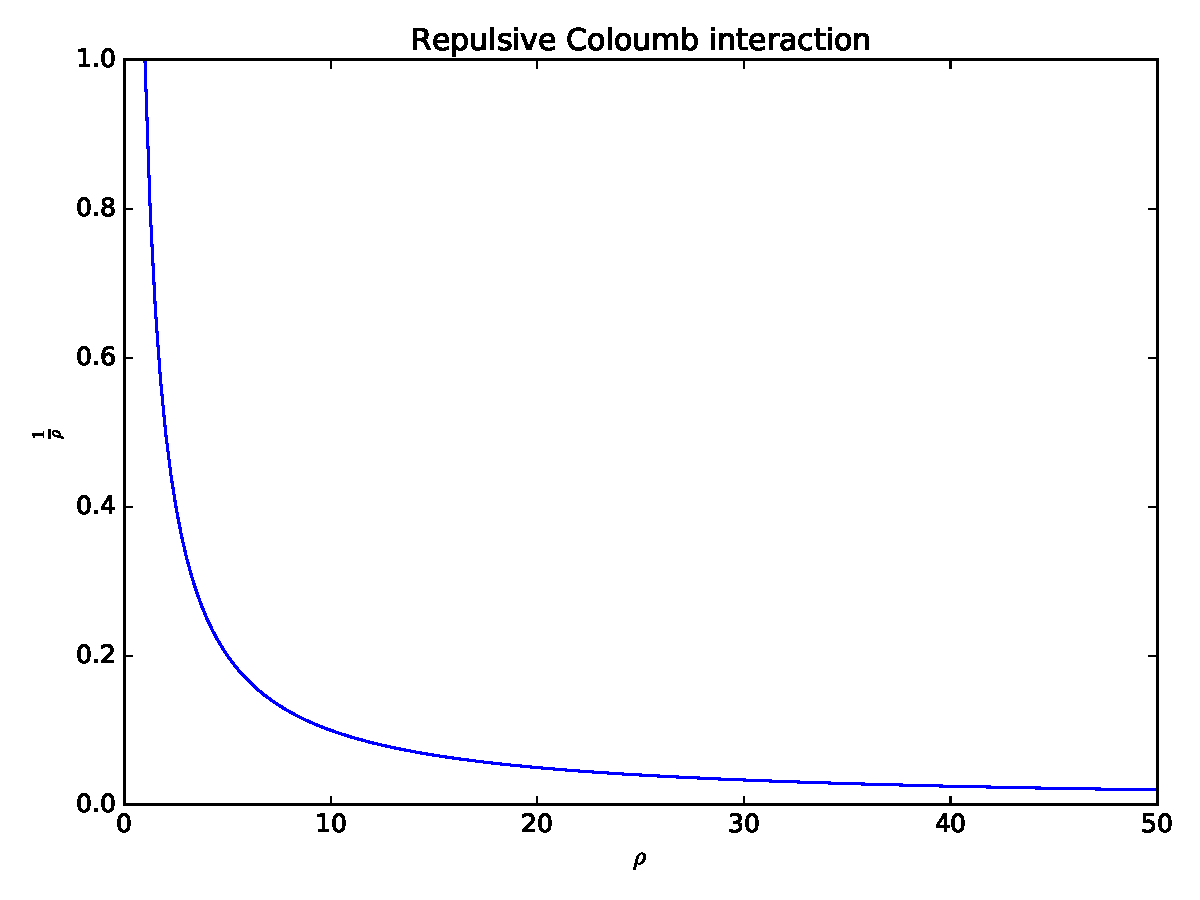
\includegraphics[width=0.8\linewidth]{fig/Repulsion.pdf}
    \caption{Repulsive Coloumb interaction}
    \label{fig:repulsion}
\end{figure}


\subsection{The numerical solution}
Discretization of the fomula in equation \ref{eq:schrodinger} and applying the three point formula in \cite{lectures} to get a numerical approximation to the second order derivate yields:

\begin{equation}
-\frac{u_{i+1} - 2u_i + u_{i-1}}{h^2} + V_iu(\rho_i) = \lambda u(\rho_i) \quad \text{ for $i=1,2,...,n$}
\end{equation}
with 

\begin{equation}
V_i=\rho_i^2
\label{eq:pot_one}
\end{equation}
for the one electron case,

\begin{equation}
V_i=\omega_r^2\rho_i^2
\label{eq:pot_two}
\end{equation}
for the two electron case and 

\begin{equation}
V_i=\omega_r^2\rho_i^2 + 1/r
\label{eq:pot_two_inter}
\end{equation}
for the two electron case with interaction. With $\rho_i = \rho_{max}/(n+1)$, where $\rho_{max}=\rho_{n+1} \approx \infty$ and $n$ being the number of gridpoints between the boundary conditions. This gives the following boundary conditions: $u_0(0)=u_{n+1}(\rho_{max})=0$ Writing this equation system in matrix form gives an eigenvalue problem $\bm{A}\bm{u}=\lambda \bm{u}$ with a $\bm{A}$ being a tridiagonal matrix:

\begin{equation}
\bm{A}=
\begin{bmatrix}
\frac{2}{h^2} + V_1 & -\frac{1}{h^2}      & 0                   & \cdots         & \cdots         & \cdots                  & 0      \\
-\frac{1}{h^2}      & \frac{2}{h^2} + V_2 & -\frac{1}{h^2}      & 0              & \cdots         & \cdots                  & 0      \\
0                   & -\frac{1}{h^2}      & \frac{2}{h^2} + V_3 & -\frac{1}{h^2} & 0              & \cdots                  & 0      \\
\vdots              & \vdots              & \ddots              & \ddots         & \ddots         & \vdots                  & \vdots \\
\vdots              & \vdots              & \vdots              & \ddots         & \ddots         & \ddots                  & \vdots \\
0                   & \cdots              & \cdots              & 0              & -\frac{1}{h^2} & \frac{2}{h^2} + V_{n-1} & -\frac{1}{h^2} \\
0                   & \cdots              & \cdots              & \cdots         & 0              & -\frac{1}{h^2}          & \frac{2}{h^2} + V_n    \\
\end{bmatrix}
\end{equation}
Such an eigenvalue problem has the property that $\det(\bm{A})=\lambda_1\lambda_2...\lambda_n$. By transforming the matrix $\bm{A}$ into a diagonal matrix finding the eigenvalues becomes trivial. 

\subsubsection{Jacobi's algorithm}
One famous method for transforming $\bm{A}$ into a diagonal matrix $\bm{D}$ is Jacobi's method. An ortogonal transformation $\bm{S}$ such that $\bm{S}^T\bm{A}\bm{S}=\bm{D}$ exists if $\bm{A}$ is real and symmetric according to \cite{lectures}. In Jacobi's method $\bm{S}$ is found by performing a series of orthogonal similarity transformations such that $\bm{S}=\bm{S}_1\bm{S}_2...\bm{S}_{m-1}\bm{S}_m$. Each transformation $\bm{S}_j$ aims to set one off-diagonal element to zero and the transformed matrix is therefore similar to the original matrix, giving the name of the transformation.

$\bm{S}_j$ is given by

\begin{equation}
\bm{S}_j=
\begin{bmatrix}
1      & 0      & \cdots      & 0           & 0         & \cdots & 0      & 0          \\
0      & 1      & \cdots      & 0           & 0         & \cdots & 0      & 0          \\
\vdots & \vdots & \ddots      & \vdots      & \vdots    & \vdots & \vdots & \vdots     \\
0      & 0      & \cdots      & \cos\theta  & \cdots    & \cdots & 0      & \sin\theta \\
0      & 0      & \cdots      & 0           & 1         & \cdots & 0      & 0          \\
0      & 0      & \cdots      & 0           & 0         & \ddots & 0      & 0          \\
\vdots & \vdots & \vdots      & \vdots      & \vdots    & \vdots & \ddots & \vdots     \\
0      & 0      & \cdots      & -\sin\theta & 0         & 0      & 0      & \cos\theta \\
\end{bmatrix}
\end{equation}
where element $s_{kk}=s_{ll}=\cos\theta$, $s_{kl}=\sin\theta$ and $s_{lk}=-\sin\theta$ are the only elements different from an identity matrix. The purpose of Jacobi's algorithm is to choose the angle $\theta$ such that element $a_{kl}=a_{lk}=0$ after the transformation. This transformation alters the elements $a_{ik}$ and $a_{il}$ for all $i=1,..n$ and an element that was previously set to zero may be changed. At a minimum $n(n-1)/2$ such similiarity transformations are needed, but more is usually needed. However, as long as the matrix $\bm{A}$ is irreducibly diagonally dominant, Jacobi's method is guaranteed to converge, according to \cite{lectures}.

As shown in \cite{lectures}, the fewest similarity transformations are needed when, for each iteration the element $a_{kl}$ chosen is the largest (absolute) off-diagonal element. However, finding the largest (absolute) off-diagonal element is a operation that scales as $\mathcal{O}(n^2)$ since the whole upper or lower triangular part of the matrix needs to be searched. 

The Jacobi transformation preserves the eigenvalues of the original eigenvalue problem $\bm{A}\bm{u}=\lambda \bm{u}$, but the eigenvectors are changed. This can be seen by rewriting the eigenvalue problem, by multiplying on the left side with $\bm{S}^T$ and inserting $\bm{S}\bm{S}^T=\bm{I}$ between $\bm{A}$ and $\bm{u}$, into:

\begin{flalign*}
\bm{S}^T\bm{A}\bm{S}\bm{S}^T\bm{u} &= \bm{S}^T\lambda\bm{u}\\
(\bm{S}^T\bm{A}\bm{S})(\bm{S}^T\bm{u}) &= \lambda(\bm{S}^T\bm{u})\\
\bm{D}(\bm{S}^T\bm{u}) &= \lambda(\bm{S}^T\bm{u})
\end{flalign*}

To start the algorithm an ortogonal vector basis $\bm{U}$ is needed. The obvious choice is to choose $\bm{U}=\bm{I}$. 

\subsubsection{Validation of results}

Given a basis of vectors $\bm{v}_i=[v_{i1} v_{i2} \hdots v_{in}]^T$, this basis is orthogonal if $\bm{v}_j^T\bm{v}_i = \delta_{ij}$, where $\delta_{ij}$ is the Kronecker delta function: 

\begin{equation*}
\delta_{ij} = 
\begin{cases}
1, &         \text{if } i=j     \\
0, &         \text{if } i\neq j \\
\end{cases}
\end{equation*}

Assuming $\bm{U}$ is an orthogonal transformation $\bm{U}$ then has the following property: $\bm{U}^T\bm{U}=\bm{I}$. Taking the dot product of a transformed vector basis $\bm{w}_i=\bm{U}\bm{v}_i$ gives:

\begin{equation*}
\bm{w}_j^T\bm{w}_i = (\bm{U}\bm{v}_i)^T(\bm{U}\bm{v}_i) = \bm{v}_i^T\bm{U}^T\bm{U}\bm{v}_i = \bm{v}_i^T\bm{I}\bm{v}_i = \bm{v}_i^T\bm{v}_i = \delta_{ij}.
\end{equation*}
This shows that the transformed vector basis $\bm{w}_i$ has preserved the dot product and is therefore also orthogonal. Since Jacobi's algorithm applies a series of orthogonal transformations on the vector basis $\bm{U}=\bm{I}$, tests can be performed to see if the orthogonality is maintained during or after the method is complete. This is a good indication of whether the algorithm is implenent correctly or whether the implementation is numerically stable.


\section{Results}
\label{sec:results}
The source code for this project is located at http://github.com/annsilje/fys3150. All the scenarios have been executed with $n=400$. This seems sufficient to get decent eigenvalues for all the chosen values of $\rho_{max}$, even though a smaller $n$ could have been used for the smaller $\rho_{max}$. Higher $n$ will yield higher precision, but will also increase execution time dramatically. Choosing $n=400$ is a reasonable compromise between execution time and precision for the purpose of this project.

\subsubsection{The physical interpretation}

Figure \ref{fig:one} shows the probablilty distributions for the three lowest lying states for the case of one electron in a harmonic oscillator well. Here, $\infty$ is approximated with $\rho_{max}=10$, which seems reasonable as the probablility distributions go towards zero shortly after $\rho=4$. This case will serve as a reference for the behaviour of the two electrons cases.

\begin{figure}[h]
    \centering
    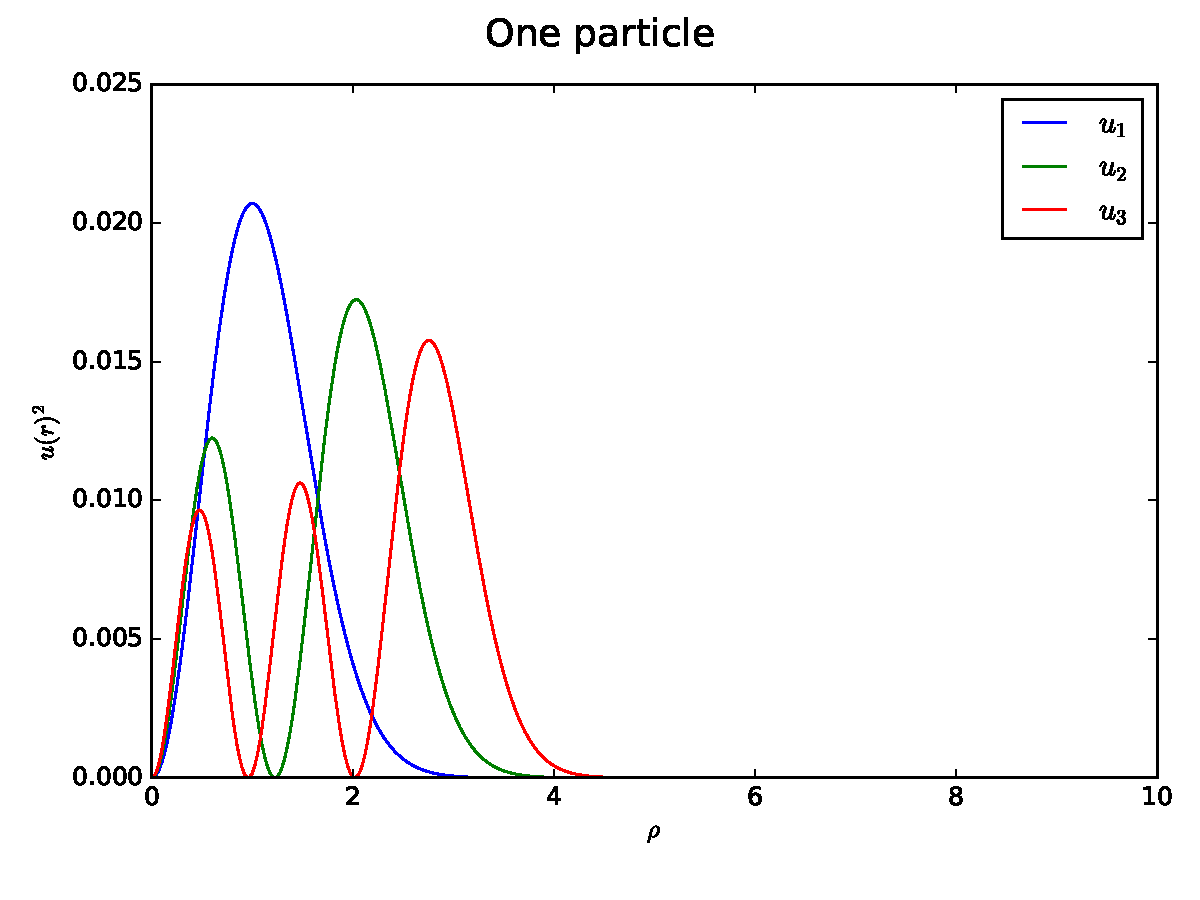
\includegraphics[width=0.8\linewidth]{fig/One_particle.pdf}
    \caption{Radial probability distributions for three lowest-lying states of one electron in a harmonic oscillator well.}
    \label{fig:one}
\end{figure}

Figure \ref{fig:two} shows the probability distributions for the three lowest lying states for two electrons in a harmonic oscillator well with no interaction between the electrons. Comparing the potential function in equation \ref{eq:pot_two} with the potential function in \ref{eq:pot_one}, with $\omega_r=1.00$ this case should be equal to the one electron case. Figure \ref{fig:two} indicates that is is correct. As $\omega_r$ becomes smaller the harmonic oscillator well becomes larger and the distance between the electrons are more likely to be larger. Similary, for higher values of $\omega_r$ the distance is more likely to be shorter as can be seen in figure \ref{fig:two}.

\begin{figure}[h]
    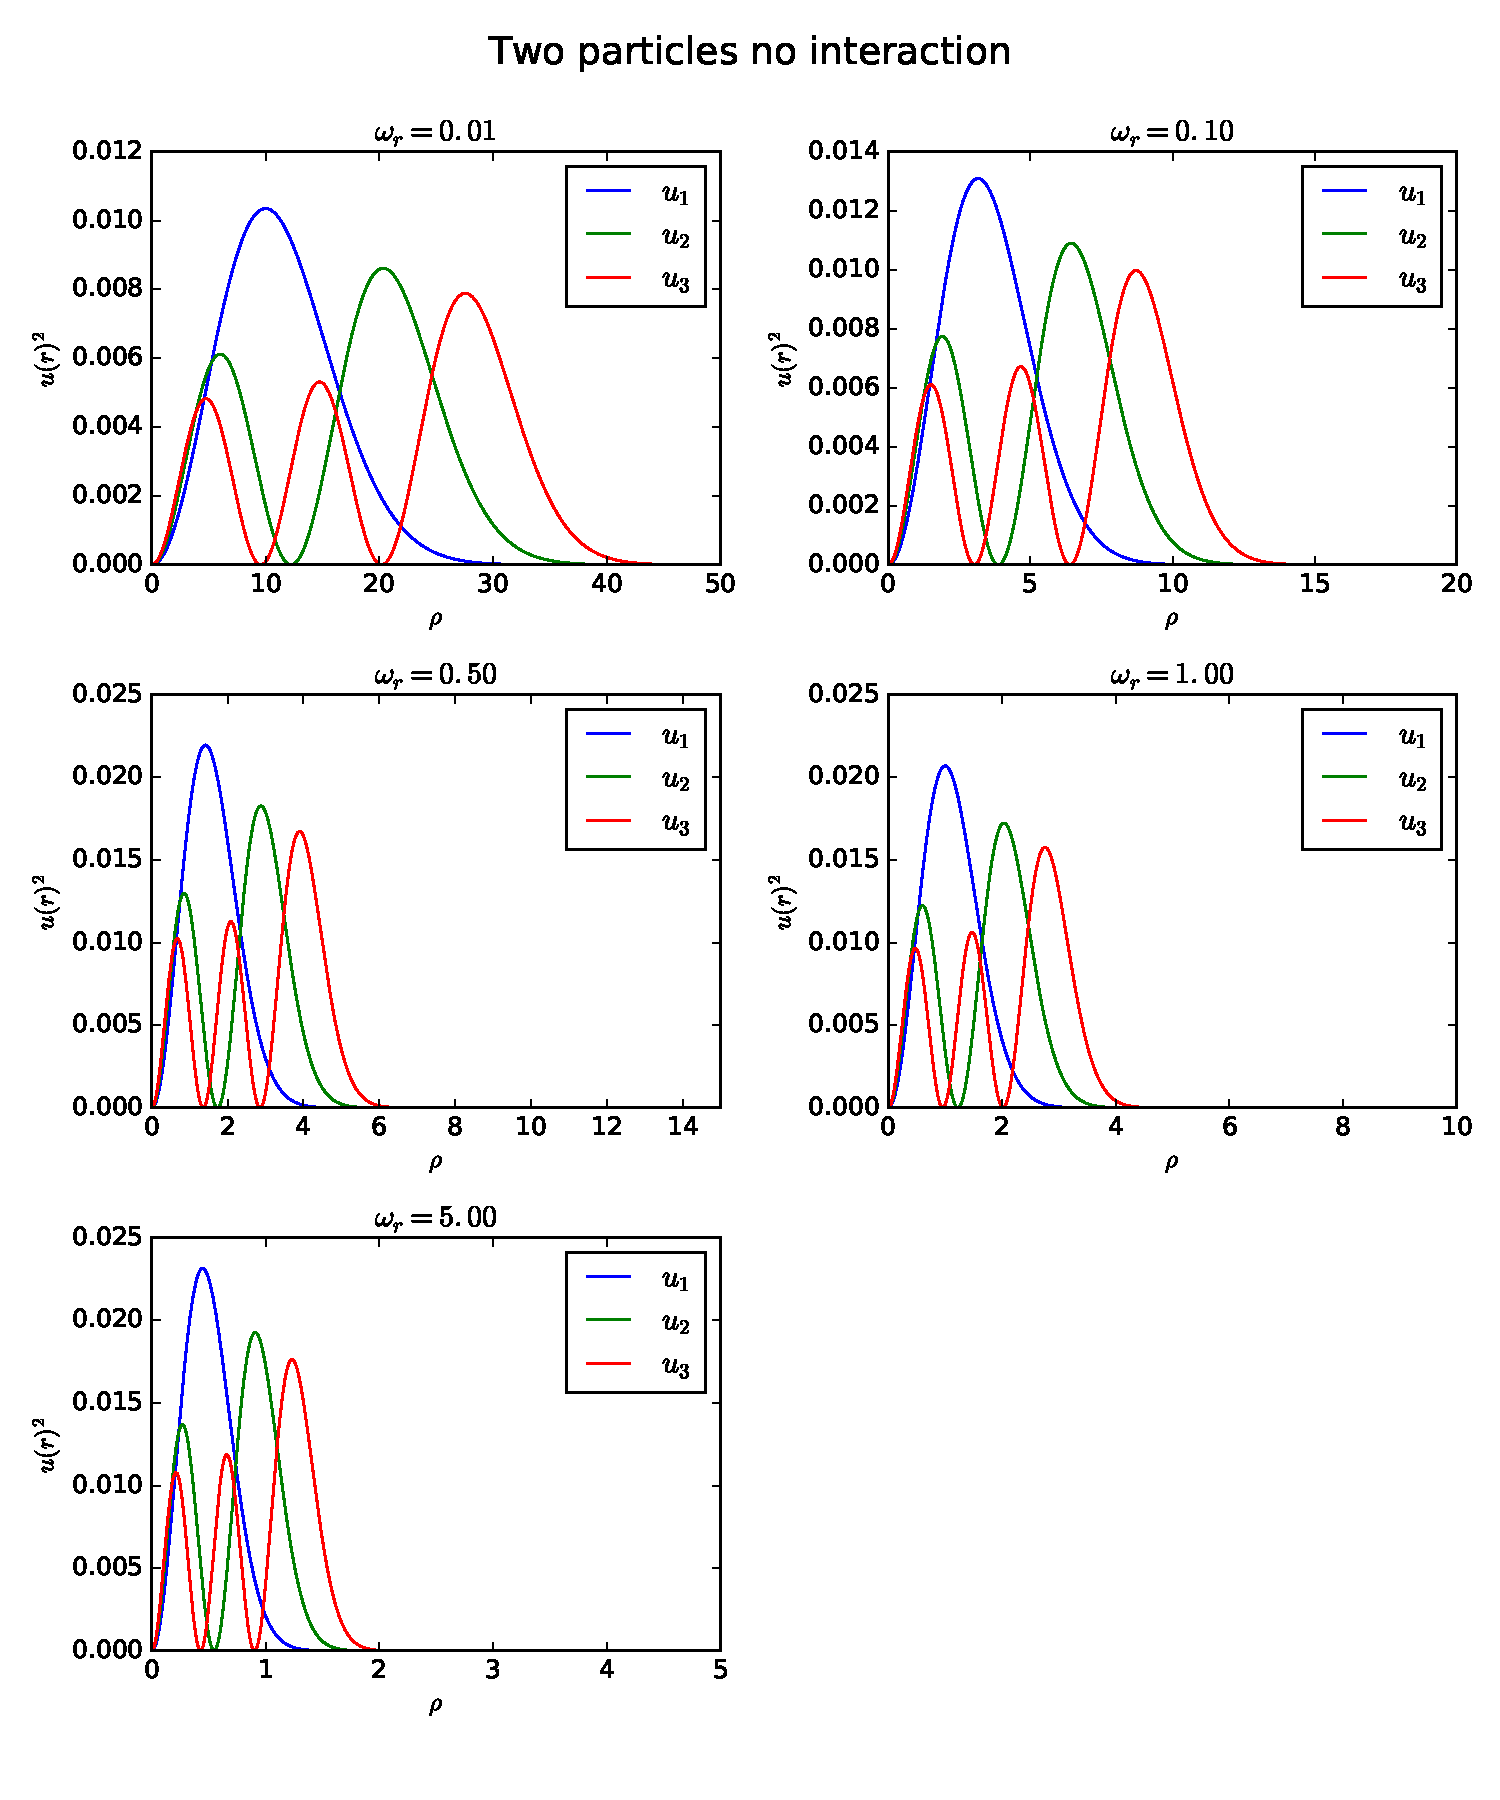
\includegraphics[width=\linewidth]{fig/Two_particles_no_interaction.pdf}
    \caption{Radial probability distributions for three lowest-lying states of two electrons in a harmonic oscillator well.}
    \label{fig:two}
\end{figure}

Figure \ref{fig:two_inter} shows the probability distributions for the three lowest lying states for two electrons in a harmonic oscillator well with repulsive Coloumb interaction. The same pattern can be seen as in the case without the repulsion, with the electrons moving further apart the wider the harmonic oscillator well becomes. 

\begin{figure}[h]
    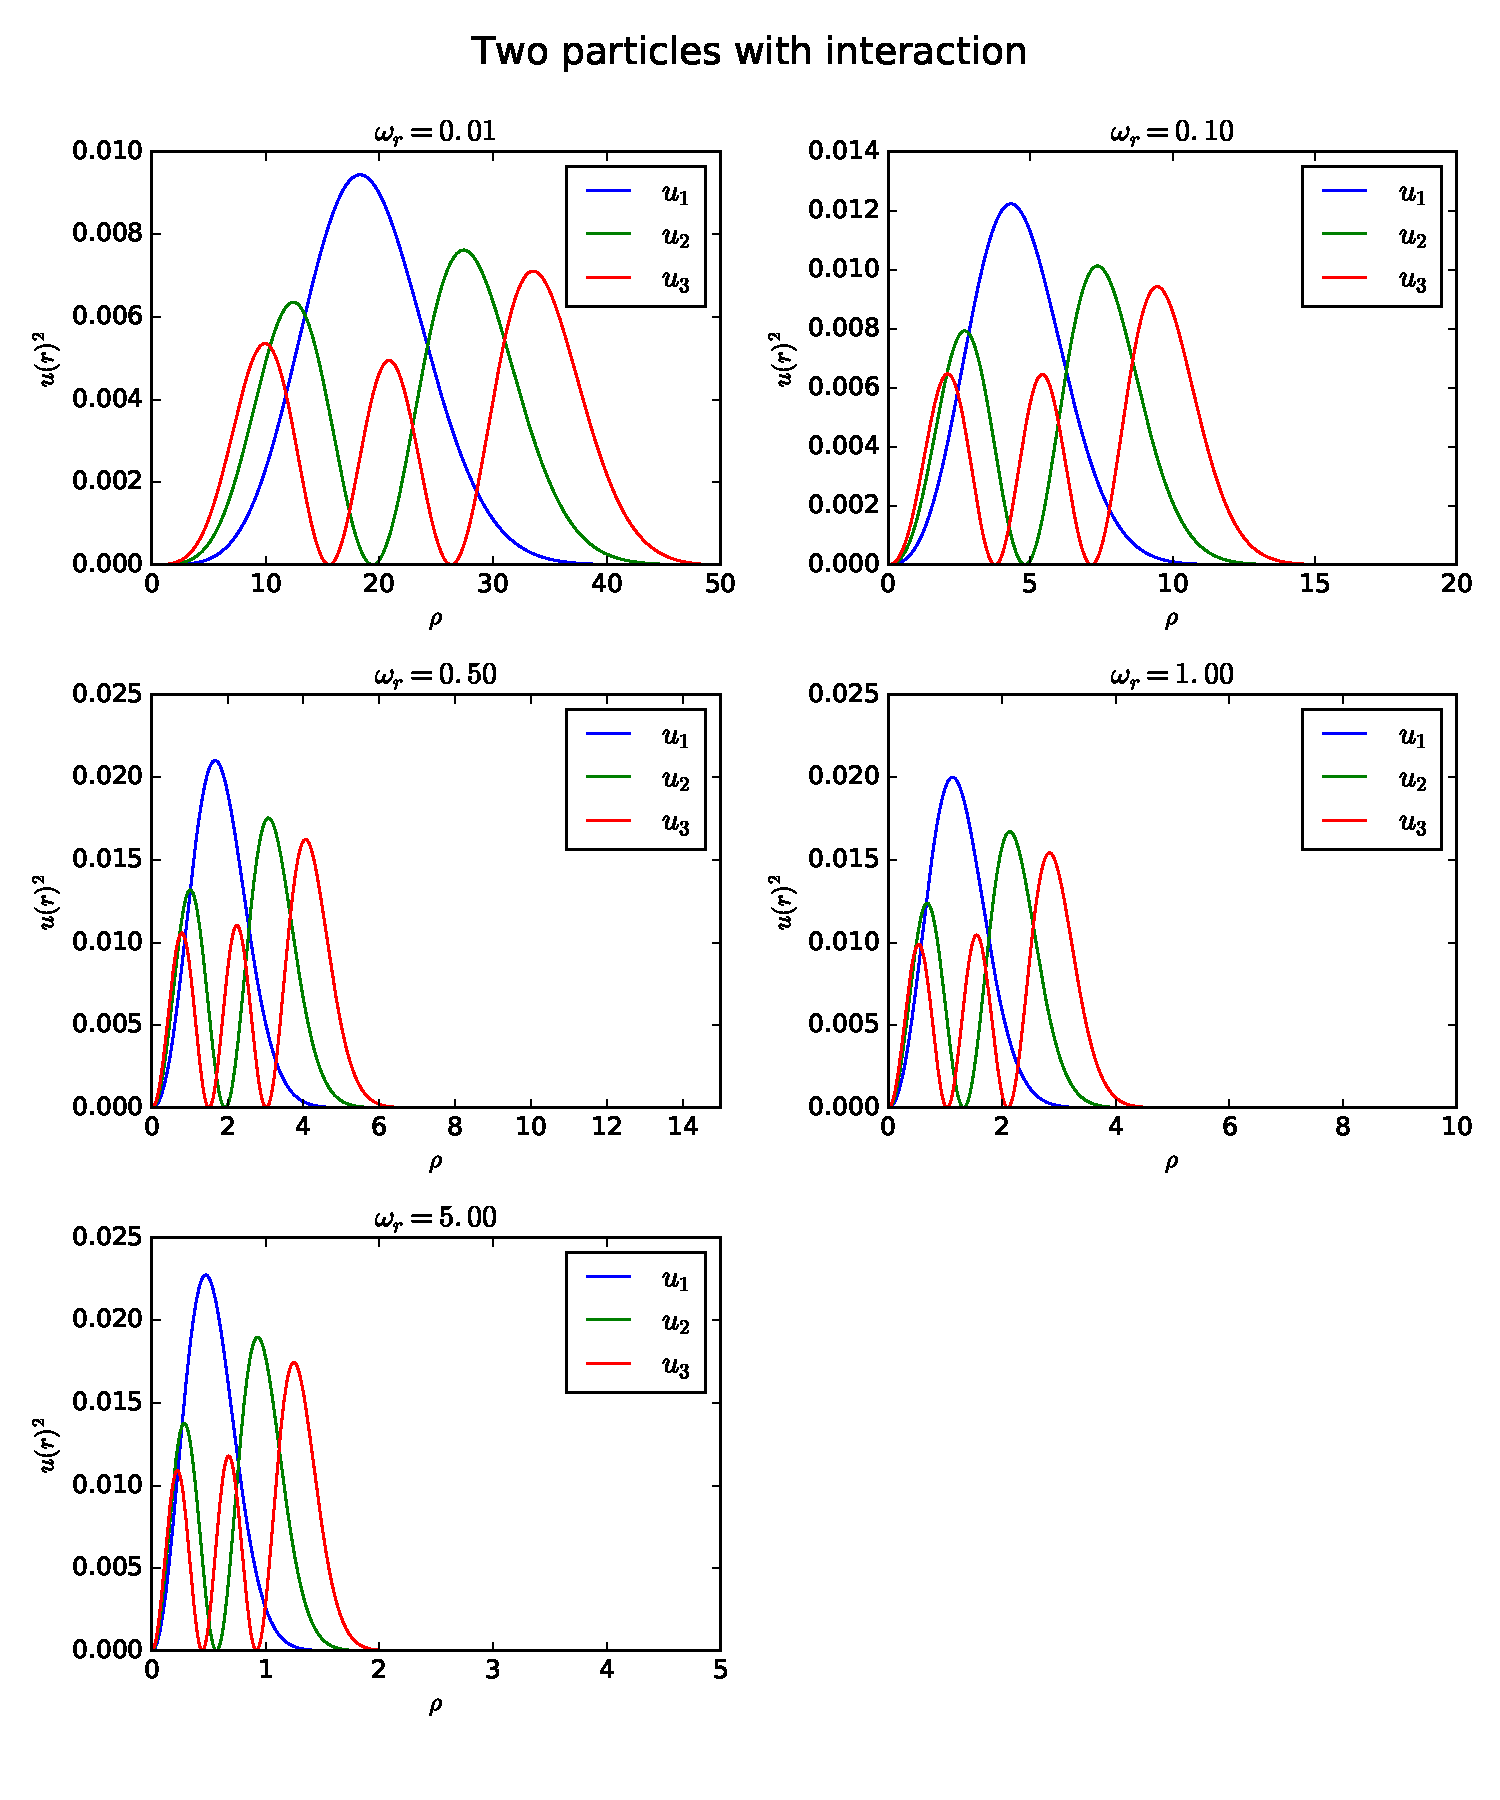
\includegraphics[width=\linewidth]{fig/Two_particles_with_interaction.pdf}
    \caption{Radial probability distributions for three lowest-lying states of two electrons in a harmonic oscillator well with interactive Coloumb repulsion.}
    \label{fig:two_inter}
\end{figure}

For the narrow well with $\omega_r=5.00$ there is not a noticable difference in the probability distribution between the two cases. However, as the harmonic oscillator well widens the more likely distance between the electrons increase. A tiny hint of this effect can be seen for $\omega_r=0.50$, but it becomes clearer with $\omega_r=0.10$ and $\omega_r=0.01$.

As shown in figure \ref{fig:repulsion} the Coloumb interaction is stronger over short distances, while these results indicate that the effects of the repulsion is only visible over larger distances. This seems to indicate that the relative strength of the repulsion compared to the harmonic oscillator well is weak for the narrow wells, but becomes stronger for the wider wells. This is probably due to the fact that even though the repulsive Coloumb interaction goes towards zero as $\rho$ goes to infinity it does so very slowly, and will therefore still be significant for the values of $\rho$ considered in this project. 

\FloatBarrier
\subsubsection{The numerical performance}

Table \ref{tab:exec} shows the execution times and the number of iterations needed for Jacobi's method to converge. 

With $n=400$ there is a totalt of 79800 off-diagonal elements that needs to be set to zero. Jacobi's method does not consider the fact that the matrix is already tridiagonal with only $n-1=399$ off-diagonal elements that are different from zero to begin with. Even with this ideal starting point the Jacobi's algorithm seem to need about 270 000 iterations on average, more than 3 times the number of off-diagonal elements in the upper or lower triangular part of matrix $\bm{A}$. This is also approximately 675 times the dimensionality of the problem.

These numbers all come from the same matrix $\bm{A}$ and might yield slightly different results for a different matricies, but the main conlusion is still that Jacobi's method is extremely slow. Comparing the execution time with a generic algorithm \texttt{arma::eig\_sym} for dense symmetric matrices implemented in the library armadillo from \cite{arma} this conclusion becomes even more evident.

\begin{table}[h]
\centering
\caption{Execution times and number of required similarity transformations.}
\label{tab:exec}
\begin{tabularx}{\textwidth}{l r r r r r r }
\hline
Case & $\omega_r$ & Step Length & $\rho_{max}$ & Iterations & Jacobi & eig\_sym\\
\hline\hline
One electron &   & $2.49 \times 10^{-2}$ & 10 & 279133 &  182.45s &  0.0155s  \\
No interaction & 0.01 & $1.25 \times 10^{-1}$ & 50 & 269020 &  176.28s &  0.0157s  \\
No interaction & 0.10 & $4.99 \times 10^{-2}$ & 20 & 276436 &  182.84s &  0.0156s  \\
No interaction & 0.50 & $3.74 \times 10^{-2}$ & 15 & 275785 &  187.76s &  0.0157s  \\
No interaction & 1.00 & $2.49 \times 10^{-2}$ & 10 & 279133 &  185.11s &  0.0157s  \\
No interaction & 5.00 & $1.25 \times 10^{-2}$ &  5 & 283636 &  191.30s &  0.0157s  \\
Interaction & 0.01 & $1.25 \times 10^{-1}$ & 50 & 270052 &  184.77s &  0.0157s  \\
Interaction & 0.10 & $4.99 \times 10^{-2}$ & 20 & 276727 &  194.84s &  0.0153s  \\
Interaction & 0.50 & $3.74 \times 10^{-2}$ & 15 & 276323 &  180.70s &  0.0159s  \\
Interaction & 1.00 & $2.49 \times 10^{-2}$ & 10 & 279901 &  187.07s &  0.0156s  \\
Interaction & 5.00 & $1.25 \times 10^{-2}$ &  5 & 283277 &  180.11s &  0.0156s  \\
\hline
\end{tabularx}
\end{table}

Table \ref{tab:comp} shows how many of the eigenvalues found with Jacobi's method are equal to the eigenvalues found with the algorithm \texttt{arma:eig\_sym}. The obvious trend is that the number of equal eigenvalues are higher for smaller $\omega_r$ and decreases as $\omega_r$ increases. The repulsive Coloumb interaction does not seem to have any effect at all. Without any information about how \texttt{arma:eig\_sym} is implemented is difficult to draw any conclusion from this, but for the three lowest lying states that are considered in this project these two methods give comparable results.

\begin{table}[h]
\centering
\caption{Number of eigenvalues that are equal when comparing Jacobi's method to \texttt{arma::eig\_sym} and the value of the three lowest eigenvalues.}
\label{tab:comp}
\begin{tabularx}{\textwidth}{l r r r r r}
\hline
Case & $\omega_r$ & Equal eigenvalues & $\lambda_1$ & $\lambda_2$ & $\lambda_3$\\
\hline\hline
One electron   &      & 146 & 2.9998 & 6.9990 & 10.9976 \\
No interaction & 0.01 & 400 & 0.0300 & 0.0700 & 0.1100\\
No interaction & 0.10 & 383 & 0.3000 & 0.7000 & 1.0999\\
No interaction & 0.50 & 240 & 1.4999 & 3.4995 & 5.4987\\
No interaction & 1.00 & 146 & 2.9998 & 6.9990 & 10.9976\\
No interaction & 5.00 & 64  & 14.9988 & 34.9939 & 54.9852\\
Interaction    & 0.01 & 400 & 0.1058 & 0.1415 & 0.1780\\
Interaction    & 0.10 & 383 & 0.5988 & 0.9683 & 1.3466\\
Interaction    & 0.50 & 240 & 2.2300 & 4.1340 & 6.0727\\
Interaction    & 1.00 & 146 & 4.0577 & 7.9087 & 11.8169\\
Interaction    & 5.00 & 64  & 17.4474 & 37.0658 & 56.8393\\
\hline
\end{tabularx}
\end{table}

\section{Conclusions}
\label{sec:conclusions}

The results indicate that with a wide harmonic oscillator well two electrons are more likely to be further apart and even further apart when the repulsive Coloumb interaction is considered. However, contrary to what one might expect the repulsive Coloumb interaction does not seem to be very significant for narrow harmonic oscillator wells.

Jacobi's method is a brute force eigenvalue problem solver that is fairly easy to implement, but is very slow and not suited for problems with dimensionality above $n=10^3$. Faster algorithms exists that gives comparable results for the lowest eigenvalues. 


%\clearpage
%\begin{appendices}
%\end{appendices}


\clearpage

\begin{thebibliography}{1}
\bibitem{lectures} Hjort-Jensen, M., 2015. Computational physics. Available at https://github.com/CompPhysics/ComputationalPhysics/
\bibitem{arma} http://arma.sourceforge.net/. C++ linear algebra library
\end{thebibliography}
\end{document}
